\documentclass[../main.tex]{subfiles}

\begin{document}

\chapter{“Luồng run rẩy mới” trong thơ Baudelaire}

\begin{metadata}

\begin{flushright}8.7.2008\end{flushright}

Hoàng Hưng

Nguồn: Kiến thức Ngày nay 10.2.2008

\end{metadata}

\begin{multicols}{2}

Có một lần, khi viết về Baudalaire, thi hào Victor Hugo lưu ý đến “luồng run rẩy mới” (un frisson nouveau) trong \textit{Ác hoa} (Les fleurs du mal) của nhà thơ này… 
 
 \begin{figure}
	\centering
	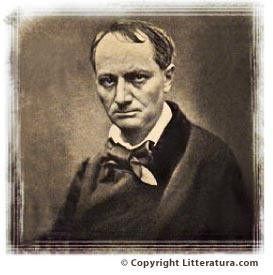
\includegraphics[width=\textwidth]{../img/tho080708_1.jpg}
	\caption{Chân dung Baudelaire}
\end{figure}
 Baudelaire phong phú hơn những gì ta có thể nghĩ về ông. Trong những bài thơ để đời của ông, nếu "Chim hải âu" (L'Albatros) là một hình tượng mang tính lãng mạn về bản chất "trên trời" của thi sĩ, thì "Cái đẹp" (La Beauté) lại là pho tượng tạc nên sự yên bình trang trọng của "giấc mơ bằng đá" đượm màu hình thức chủ nghĩa của phái Thi Sơn (Parnasse). Và với tất cả sự chính xác của từ ngữ, sự vững chãi của cấu trúc, sự hoàn chỉnh về kỹ thuật thể điệu và hình thức thơ nói chung, Baudelaire cũng được coi như một nhà thơ "cổ điển". 
 
Thế nhưng \textit{Ác hoa} của nhà thơ (ra mắt năm 1857, tái bản bổ sung 1861, tái bản sau khi tác giả qua đời và được bổ sung khá nhiều năm 1866) đã là một cơn động đất trong thơ Pháp, rồi còn trở thành nguyên khởi cho một thứ mà nhà phê bình Sainte-Beuve gọi là "Cơn điên Baudelaire" (La Folie Baudelaire), và một trong các tác nhân tạo nên "Bệnh Thế kỷ" (le Mal du Sìecle) vào cuối thế kỷ XX.  
 
Những "cơn" ấy được thổi lên từ "luồng run rẩy mới" mà Hugo nói. 
 
 
\textbf{Người tiên phong của chủ nghĩa tượng trưng (Symbolisme)} 
 
Khái niệm Symbolisme chỉ xuất hiện mãi vào năm 1886 trong \textit{Tuyên ngôn }của nhà thơ Jean Moréas sau khi ba cái tên Verlaine, Rimbaud và Mallarmé đã nổi như cồn. Symbolisme theo Moréas là phương pháp nghệ thuật tìm cách \textbf{khơi gợi, bằng hiệu quả âm nhạc và tượng trưng của từ ngữ}, những cung bậc tinh tế nhất của cảm nhận và các trạng thái tâm hồn. Nó gắn bó với \textbf{sự bí nhiệm }và \textbf{cốt tủy tâm linh }của mọi người mọi vật, tìm cách tạo nên những "cái tương đương mang tính tạo hình" của tự nhiên và tư tưởng.  
 
Từ đó nhìn lại Baudelaire, người ta coi ông là người tiên phong của chủ nghĩa tượng trưng. (Gerard de Nerval ở Pháp và Edgar A. Poe ở Mỹ được coi như những "người báo trước" - les précurseurs.) 
 
Hãy đọc lại bài thơ mà hầu như ai cũng dẫn ra của Baudelaire để minh hoạ cho những quan niệm "tượng trưng chủ nghĩa" của nhà thơ này: 
\begin{blockquote}
        
TƯƠNG ỨNG (CORRESPONDANCES) 
        
Thiên nhiên là ngôi đền mà các cột trụ sống        
Đôi khi để lọt ra những lời nói tối nghĩa         
Con người đi qua đó xuyên những khu rừng biểu tượng        
Chúng quan sát anh ta với những cái nhìn thân quen 
        
Giống như những tiếng vang kéo dài, lẫn vào nhau từ xa        
Trong sự hợp nhất tối tăm và sâu thẳm        
Rộng như đêm và như ánh sáng        
Các hương thơm, màu sắc và âm thanh đáp lời nhau 
        
Có những mùi hương tươi mát như da thịt trẻ con,        
Êm như kèn ôboa, xanh ngắt như đồng cỏ,        
- Và những mùi hương khác, hư đốn, giàu có và chiến thắng 
        
Có sức tràn lan của những vật vô tận        
Như long diên hương, xạ hương, an tức hương (benjoin), hương nhựa \textit{boswellia}        
Chúng ca lên những rung cảm của tâm trí và các giác quan  

\end{blockquote}
 
Phải nói ngay rằng khái niệm "biểu tượng" trong bài thơ này không có gì giống với thư thủ pháp ngôn ngữ sử dụng thi ảnh để tượng trưng một ý niệm (kiểu như "biểu tượng hai mặt" mà ta quen nghe trong một thời kỳ đấu tranh văn học nặng nề), mà đây là những ký hiệu trong đời sống tự nhiên ẩn giấu một thông điệp bí nhiệm của cái Đẹp, của cái Siêu nhiên mà con người khát khao khám phá. Như Baudelaire nói trong bài thơ vừa dẫn, "thiên nhiên" chỉ là "ngôi đền" "để lọt ra những lời nói tối nghĩa" mà ta phải giải mã để đạt đến sự cộng thông với cái ở trên cõi cao vời, cái Thần linh.\textit{"Chính cái bản năng tuyệt vời về cái Đẹp khiến chúng ta coi trái đất và những cảnh trí của nó như một hình ảnh đại quát của trời cao, như một sự tương ứng với trời cao. Chính vừa bởi thơ ca vừa thông qua thơ ca, bởi âm nhạc và thông qua âm nhạc, mà hồn ta hé thấy những vẻ huy hoàng nằm ở phía sau nấm mộ." }(Baudelaire - Những bài viết về Theophile Gautier). 
 
Ở thời đại ngày nay, khi nhận thức về sự tồn tại của thế giới hữu hình và thế giới vô hình, thế giới vật chất và thế giới tâm linh đã không còn xa lạ với chúng ta, thì quan niệm của Baudelaire về "biểu tượng" chẳng có gì khó hiểu. 
 
Làm thế nào để đọc được những biểu tượng ấy?  
 
Baudelaire chỉ ra rằng:\textit{ "Làm bốc hơi và tập trung cao độ cái Tôi. Tất cả là ở đó" }(Trích \textit{Nhật ký tác giả}). 
 
"Làm bốc hơi cái Tôi" cũng có nghĩa là đạt đến sự xuất thần.  
 
Xuất thần để cảm nhận được sự tương ứng của các tín hiệu, "những tiếng vang kéo dài lẫn vào nhau từ xa, trong sự hợp nhất tối tăm và sâu thẳm, rộng như đêm và như ánh sáng, các hương thơm, màu sắc và âm thanh đáp lời nhau". 
 
Cần nói thêm là trong những cảm giác tương ứng trên, Baudelaire đặc biệt nhạy với các mùi hương - loại cảm giác có hiệu ứng kích thích xác thịt, trong khi Verlaine thường để hồn tan trong âm nhạc ("Âm nhạc là trước tất cả mọi điều") là thứ gợi những cảm xúc trừu tượng nhiều hơn. 
 
Cái Đẹp tuyệt đối, cái Siêu nhiên mà Baudelaire nói tới thật ra cũng chưa bao giờ được ông trao gửi người đọc một cách thuyết phục. Ở những vần thơ trong lành nhất của ông, ta cũng chỉ cảm nhận mơ hồ một thế giới trên "tầng thượng thanh khí" (xin lưu ý đến từ này trong thơ Hàn Mặc Tử), ở đó có "thứ lửa sáng tràn ngập các khoảng khống trong vắt" giống như "một thứ rượu ngọt thuần khiết và thần thánh" (“Cao thượng”). 
 
Ta cũng phải thừa nhận rằng, để đạt sự xuất thần, cũng giống như Edgar Poe mà ông chịu ảnh hưởng, Baudelaire đã tìm đến "Những thiên đường nhân tạo" (tên một cuốn sách phân tích các trải nghiệm của bản thân tác giả). Ông đã là một đệ tử của rượu, cần sa và cồn thuốc phiện (laudanum). "Thiên đường" của ông được miêu tả khá rõ trong bài thơ xuôi "Căn phòng đôi" (trích trong tập \textit{Chứng u sầu Paris} (Spleen de Paris): "Một căn phòng giống như sự mơ màng, một căn phòng thực sự thuộc về thế giơi tinh thần mà không khí thì ngưng đọng và phơn phớt hồng lam… Tâm hồn ở đó tắm trong sự biếng lười, phảng phất mùi hương tiếc nuối và thèm muốn… Thời gian đã biến mất, chính là sự vĩnh hằng ngự trị, một sự vĩnh hằng của những lạc thú." 
 
Trong một bài thơ khác ("Mời đi du ngoạn"), thiên đường của ông được hình dung là nơi "Ở đó tất cả chỉ là trật tự và cái đẹp/ Xa hoa, yên ả và khoái lạc". Cũng chỉ là một "thiên đường nhân tạo mà thôi." 
 
 
\textbf{Vẻ đẹp của cái Ác} 
 
 \begin{figure}
	\centering
	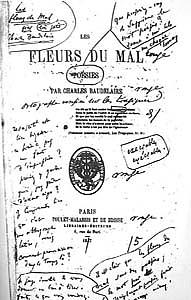
\includegraphics[width=\textwidth]{../img/tho080708_2.jpg}
	\caption{Bìa tập \textit{Fleurs du Mal} có bút tích của Baudelaire}
\end{figure}
 Người ta thường nói đến sự đối lập trong thơ Baudelaire: Thượng đế - Quỷ vương, cái Lý tưởng - cái Nhục cảm, cái Cao khiết - cái Nhơ bẩn. 
 
Paul Valery, một nhà thơ được xếp vào phái "Tượng trưng" cuối thế kỷ XIX, đã nhận định rằng thơ Baudelaire có \textit{"một sự phối kết giữa xác thịt và trí tuệ, một sự hoà trộn của long trọng, nhiệt hứng và đắng cay". }Ông cho rằng Verlaine và Rimbaud đã chịu ảnh hưởng quyết định của thơ Baudelaire ở \textit{"sự hoà trộn mãnh liệt và bối rối của cảm xúc thần bí với nóng bỏng nhục cảm… ý thức sâu xa về các cảm giác và những vang âm hài hoà của chúng".} 
 
Baudelaire có những vần thơ hướng thượng khá đẹp: 
\begin{blockquote}
        
Hãy bay lên thật xa khỏi những ám khí bệnh hoạn kia        
Hãy thanh lọc mình trong tầng thượng thanh khí 
        
Những ý nghĩ tựa như chim chiền chiện        
Tự do vút lên những tầng trời ban sớm        
Lượn bên trên cuộc đời và dễ dàng hiểu được        
Ngôn ngữ của muôn hoa và những vật lặng câm"         
        
(“Hướng thượng”) 

\end{blockquote}
 
Baudelaire có những bài thơ tuyệt đẹp về thân thể phụ nữ. Cái "toà thiên nhiên" mà Nguyễn Du chỉ với hai câu cho cảm giác về chất và khối, thì Baudelaire tạc hẳn thành tượng đài kỳ vĩ, hoành tráng. 
\begin{blockquote}
        
NÀNG KHỔNG LỒ 
        
Vào thời mà Tự nhiên đầy cao hứng        
Mỗi ngày hoài thai những đứa con quái dị        
Tôi ước mình được sống bên một cô gái khổng lồ        
Như con mèo khoái trá nằm dưới chân một nữ hoàng 
        
Tôi ước được nhìn thấy thân thể nàng nở hoa cùng với tâm hồn        
Và tự do lớn lên trong những trò chơi khủng khiếp        
Đoán xem tim nàng có ủ chăng ngọn lửa tối        
Với những dải sương ẩm ướt bơi trong mắt nàng 
        
Thoải mái dạo khắp những hình thù mỹ miều của nàng        
Trườn bò trên sườn dốc của hai đầu gối kếch xù        
Và đôi khi, giữa mùa mùa hè, khi mặt trời độc địa 
        
Khiến nàng mệt mỏi nằm xoài trên cánh đồng        
Thì tôi ngủ biếng lười dưới bóng đôi bầu vú        
Như một xóm yên bình ngủ dưới chân núi 

\end{blockquote}
 
 
 \begin{figure}
	\centering
	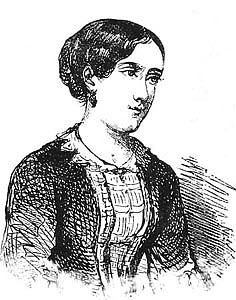
\includegraphics[width=\textwidth]{../img/tho080708_3.jpg}
	\caption{Một trong các "nàng Thơ" của Baudelaire}
\end{figure}
 Cô gái lai phong nhiêu Jeanne Duval được coi là nàng thơ của bài thơ độc đáo này. 
 
Nhưng phải nói thực rằng tai tiếng mà \textit{Ác hoa} gây nên chính là do tập thơ quá mạnh ở những rung cảm thuộc vế sau. Nhà thơ đã từng nói không ít về "vẻ đẹp của cái Ác" (La beauté du Mal - Từ "Mal"  dịch là "Ác" hàm nghĩa chung cái xấu, cái tiêu cực, cái đen tối, cái tà.) 
 
Những dòng sau đây trong bài thơ "Cái xác thối" có thể tiêu biểu cho cảm xúc về cái xấu, cái nhơ nhớp: 
\begin{blockquote}
        
Và bầu trời ngắm nhìn cái xác thối tuyệt vời        
Như một bông hoa đang nở 
        
Lũ ruồi nhặng vù vù trên cái bụng thối        
Từ đó tuôn ra đen ngòm những đoàn quân ròi        
Rồi chảy xuống như chất lỏng sền sệt        
Dọc theo các miếng giẻ đang động đậy 
        
Tất cả dập xuống dềnh lên như sóng        
Vừa trào lên vừa sủi bọt        
Dường như cái xác được luồng hơi mơ hồ thổi phồng lên        
Vừa cựa quậy vừa nhân thành nhiều bản… 

\end{blockquote}
 
Nếu tác giả là một Phật tử, thì ta có thể cho bài thơ là một thực hành phép "quán thân bất tịnh" nhắm cái đích diệt dục! Nhưng đây chỉ là bức tranh tưởng tượng mà tác giả vẽ lên cho người tình (có lẽ là một cô nàng kiêu kỳ với sắc đẹp của mình) hình dung cái gì còn lại của một thân xác mỹ miều, vì kết thúc bài thơ là lời nhắn nhủ: 
\begin{blockquote}
        
Khi đó người đẹp ơi, hãy nói cùng ròi bọ        
Đang ăn người bằng những chiếc hôn        
Rằng anh đã giữ lại hình và cốt        
Của những cuộc tình đã bị hủy phân. 

\end{blockquote}
 
Một bức tranh kinh dị khác miêu tả bộ mặt ma cà rồng của người đẹp trong ân ái (trích từ một trong sáu bài thơ bị tòa án tuyên phạt vì xâm phạm mỹ tục và phải loại bỏ ở lần tái bản thứ hai, đến lần tái bản thứ ba mới đưa vào trở lại): 
\begin{blockquote}
        
Người đàn bà, từ cái miệng mát ngọt như dâu tây        
Vừa vặn mình như con rắn trên than hồng        
Vừa nắn bóp cặp vú thòi trên gọng cooc xê        
Tuôn ra những lời đượm mùi hương xạ: 
        
"Ta, ta có cặp môi ẩm ướt và ta nắm được khoa học        
Làm cho ý thức cổ lỗ mất tiêu trên một cái giường        
Ta làm khô tất cả nước mắt trên cặp vú chiến thắng của ta        
Và làm cho các lão già cười lên tiếng cười con trẻ        
Ta thay thế, cho những ai nhìn thấy ta trần truồng không mảnh vải        
Cả mặt trời, mặt trăng, bầu trời với những vì sao!        
Nhà bác học thân mến ơi, ta quá thông thái về các môn khoái lạc        
Mỗi khi ta làm nghẹt thở một gã đàn ông trong đôi tay đáng sợ của ta        
Hay khi, cho những vết cắn, ta buông thả tấm thân        
Rụt rè và phóng túng, mảnh mai và cường tráng,        
Đến nỗi trên chăn nệm ngất ngây vì xúc động        
Các thiên thần bất lực sẽ tự chuốc lấy tội vì ta!" 
        
(“Những hoá thân của ma cà rồng”) 

\end{blockquote}
 
Chính vì những cảm hứng "đen" này mà Baudelaire và những người cùng khuynh hướng với ông được gọi là "suy đồi" (decadent). 
 
Giữa hai cực Thiện - Ác, có cả một thế giới những điều tinh tế trong bóng tối tâm hồn mà Baudelaire là người đầu tiên nắm được bí quyết diễn đạt. J. K. Huysmans, nhà văn từ bỏ chủ nghĩa tự nhiên đến với các cây bút "suy đồi" (và cuối cùng thì hướng về những cảm xúc Kitô giáo) đã viết rằng: \textit{"Trong một thời đại mà câu thơ chỉ còn phục vụ cho việc vẽ nên vẻ bề ngoài của vạn vật, Baudelaire đã đi tới chỗ \textbf{diễn đạt được cái không thể diễn đạt… }có được sức mạnh diệu kỳ trong việc diễn đạt xác đáng, một cách mạnh mẽ kỳ lạ những trạng thái bệnh hoạn khó nắm bắt nhất, bối rối nhất, của những tâm trí kiệt quệ và những tâm hồn buồn thảm."} 
 
Trong bài thơ đầu tiên của tập \textit{Ác hoa}, như một lời nhắn "Gửi bạn đọc", Baudelaire xác định rằng: giữa những thế lực đen ám ảnh con người của thời đại mình, thứ "xấu xa nhất, hung ác nhất, bẩn thỉu nhất", "con quỷ tinh tế" sẵn lòng "nuốt chửng thế giới trong một cái ngáp", chính là "Sự chán chường" (l'Ennui). 
Nó tích tụ và phát triển thành chứng bệnh mang tên "Chứng u sầu" (Spleen). Trước kẻ thù này, hy vọng chỉ có thể chiến bại: 
 \begin{figure}
	\centering
	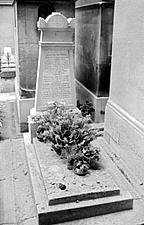
\includegraphics[width=\textwidth]{../img/tho080708_4.jpg}
	\caption{Mộ của Baudelaire có khắc hai câu thơ trên bia đá}
\end{figure}
 \begin{blockquote}
        
Những quả chuông đột nhiên nhảy thách lên        
Tung lên trời tiếng hú rùng rợn        
Giống như những linh hồn lang thang không quê hương        
Cất tiếng than van dai dẳng 
        
Và những đám tang kéo dài, không kèn không trống        
Chậm rãi diễu đi trong hồn tôi; Hy vọng        
Bại trận khóc và nỗi khắc khoải tàn bạo, chuyên chế        
Trên chiếc sọ gục xuống của tôi cắm lá cờ đen. 
        
(“Chứng u sầu”) 

\end{blockquote}
 
Tâm trạng của Baudelaire thường hợp với màn đêm, vì đó là tâm trạng gần với hư vô: 
\begin{blockquote}
        
Ta thích ngươi làm sao hỡi Đêm! Đừng có các vì sao        
Ánh sáng của chúng nói một thứ tiếng đã quen        
Vì ta đi tìm cái trống không, và cái đen và cái trần trụi!        
        
(“Ám ảnh”) 

\end{blockquote}
 
Cuối cùng, là ám ảnh của thế giới bên kia: 
\begin{blockquote}
        
Nhưng chính bóng đêm cũng là những tấm phông        
Ở đó hàng ngàn sinh linh đã khuất có cái nhìn thân thuộc        
Vọt ra từ con mắt của ta         
        
(“Ám ảnh”) 

\end{blockquote}
 
 
  Và cái chết cũng là lối thoát cuối cùng khi hy vọng đã tắt, những thiên đường trần thế không giải thoát được tác giả khỏi chứng u sầu: "Hỡi Thần chết, người thuyền trưởng già, đã đến lúc rồi! Hãy nhổ neo thôi!" (“Thần chết”) 
        
\begin{center}
*\end{center}
 
Nói gì thì nói, cứu cánh của thơ hay nghệ thuật nói chung là không ngừng khám phá nội tâm con người bằng ngôn ngữ hình tượng. Sau con người lý trí sáng suốt của chủ nghĩa cổ điển, con người tình cảm tràn bờ của chủ nghĩa lãng mạn, con người duy mỹ lạnh lùng của chủ nghĩa hình thức Thi Sơn, Baudelaire phát hiện con người bí ẩn của bóng tối vô thức, trong đó quằn quại cuộc chiến giữa cái Đẹp hướng thượng và cái bản năng ma quỷ kéo xuống bùn nhơ. Đó chính là "luồng run rẩy mới" báo hiệu cả một thời hiện đại trong thơ, khi con người biết nhìn vào không chỉ phần trên mà cả phần dưới, không chỉ phần nổi mà cả phần chìm, không chỉ mặt sáng mà cả mặt tối, để có được hình ảnh ngày càng trung thực và toàn vẹn của chính mình. 
 
\textit{Linh Đàm tháng 7 năm 2006} 
\end{multicols}
\end{document}